


%% For double-blind review submission, w/o CCS and ACM Reference (max submission space)
\documentclass[acmsmall,review,anonymous]{acmart}
\settopmatter{printfolios=true,printccs=false,printacmref=false}
%% For double-blind review submission, w/ CCS and ACM Reference
%\documentclass[acmsmall,review,anonymous]{acmart}\settopmatter{printfolios=true}
%% For single-blind review submission, w/o CCS and ACM Reference (max submission space)
%\documentclass[acmsmall,review]{acmart}\settopmatter{printfolios=true,printccs=false,printacmref=false}
%% For single-blind review submission, w/ CCS and ACM Reference
%\documentclass[acmsmall,review]{acmart}\settopmatter{printfolios=true}
%% For final camera-ready submission, w/ required CCS and ACM Reference
%\documentclass[acmsmall]{acmart}\settopmatter{}


%% Journal information
%% Supplied to authors by publisher for camera-ready submission;
%% use defaults for review submission.
\acmJournal{PACMPL}
\acmVolume{1}
\acmNumber{1} % CONF = POPL or ICFP or OOPSLA
\acmArticle{1}
\acmYear{2018}
\acmMonth{1}
\acmDOI{} % \acmDOI{10.1145/nnnnnnn.nnnnnnn}
\startPage{1}

%% Copyright information
%% Supplied to authors (based on authors' rights management selection;
%% see authors.acm.org) by publisher for camera-ready submission;
%% use 'none' for review submission.
\setcopyright{none}
%\setcopyright{acmcopyright}
%\setcopyright{acmlicensed}
%\setcopyright{rightsretained}
%\copyrightyear{2018}           %% If different from \acmYear

%% Bibliography style
\bibliographystyle{ACM-Reference-Format}
%% Citation style
%% Note: author/year citations are required for papers published as an
%% issue of PACMPL.
\citestyle{acmauthoryear}   %% For author/year citations


%%%%%%%%%%%%%%%%%%%%%%%%%%%%%%%%%%%%%%%%%%%%%%%%%%%%%%%%%%%%%%%%%%%%%%
%% Note: Authors migrating a paper from PACMPL format to traditional
%% SIGPLAN proceedings format must update the '\documentclass' and
%% topmatter commands above; see 'acmart-sigplanproc-template.tex'.
%%%%%%%%%%%%%%%%%%%%%%%%%%%%%%%%%%%%%%%%%%%%%%%%%%%%%%%%%%%%%%%%%%%%%%
%%%%%%%%%%%%%%%%%%%%%%%%%%%%%%%%%%%%%%%%%%%%%%%%%%%%%%%%%%%%%%%%%%%%%%
% our packages 
\usepackage{listings}
\usepackage{placeins}
\usepackage{multicol}

\lstset{basicstyle={\footnotesize\ttfamily},
    keywordstyle=\bfseries,
    columns=keepspacing,
    escapeinside={*@}{@*},
    firstnumber=last,
    frame=bt,
    framexleftmargin={1em},
    numbers=left,
		numberstyle={\tiny},
		stepnumber=1,
		numbersep=.7em,
    tabsize=2,
    literate={->}{{$\rightarrow$}}2
             {<|}{{$\langle$}}1
             {|>}{{$\rangle$}}1
             {<=}{{$\leq$}}1
             {>=}{{$\geq$}}1
             {!=}{{$\neq$}}1
             {@in}{{$\in$}}1
             {@iff}{{$\iff$}}1
             %{&&}{{$\land$}}1
             {EMPTY}{{$\emptyset$}}1
             %{||}{{$\lor$}}1
						 {*}{{$^*$}}1,
    commentstyle=\color{red}\itshape,
		moredelim=**[is][\color{blue}]{~}{~},
    xleftmargin={1em}}







 
% \usepackage{filecontents}
% \usepackage{xcolor}
\usepackage{xspace}

\newcommand{\todo}[1]{\textcolor{red}{{#1}}}

\newcommand{\toolname}{\textit{Leroy}\xspace}

\newcommand{\toolnamepy}{\textit{Leroy4Py}\xspace}

\newcommand{\avgcompression}{1.05x}
% Library Extraction for a Python program

% LEAP
%%%%%%%%%%%%%%%%%%%%%%%%%%%%%%%%%%%%%%%%%%%%%%%%%%%%%%%%%%%%%%%%%%%%%%

%% Some recommended packages.
\usepackage{booktabs}   %% For formal tables:
                        %% http://ctan.org/pkg/booktabs
\usepackage{subcaption} %% For complex figures with subfigures/subcaptions
                        %% http://ctan.org/pkg/subcaption


\begin{document}

%% Title information
\title{Leroy: Library Learning for Imperative Programming Languages} 
% \title[Short Title]{Full Title}         %% [Short Title] is optional;
                                        %% when present, will be used in
                                        %% header instead of Full Title.
% \titlenote{with title note}             %% \titlenote is optional;
                                        %% can be repeated if necessary;
                                        %% contents suppressed with 'anonymous'
% \subtitle{Subtitle}                     %% \subtitle is optional
% \subtitlenote{with subtitle note}       %% \subtitlenote is optional;
                                        %% can be repeated if necessary;
                                        %% contents suppressed with 'anonymous'


%% Author information
%% Contents and number of authors suppressed with 'anonymous'.
%% Each author should be introduced by \author, followed by
%% \authornote (optional), \orcid (optional), \affiliation, and
%% \email.
%% An author may have multiple affiliations and/or emails; repeat the
%% appropriate command.
%% Many elements are not rendered, but should be provided for metadata
%% extraction tools.

%% Author with single affiliation.
\author{Abhiram Bellur}
% \authornote{with author1 note}          %% \authornote is optional;
                                        %% can be repeated if necessary
% \orcid{nnnn-nnnn-nnnn-nnnn}             %% \orcid is optional
\affiliation{
  % \position{Position1}
  % \department{Department1}              %% \department is recommended
  \institution{CU Boulder}            %% \institution is required
  % \streetaddress{Street1 Address1}
  % \city{City1}
  % \state{State1}
  % \postcode{Post-Code1}
  % \country{Country1}                    %% \country is recommended
}
\email{Abhiram.Bellur@colorado.edu}          %% \email is recommended

%% Author with single affiliation.
\author{Razan Alghamdi}
% \authornote{with author1 note}          %% \authornote is optional;
                                        %% can be repeated if necessary
% \orcid{nnnn-nnnn-nnnn-nnnn}             %% \orcid is optional
\affiliation{
  % \position{Position1}
  % \department{Department1}              %% \department is recommended
  \institution{CU Boulder}            %% \institution is required
  % \streetaddress{Street1 Address1}
  % \city{City1}
  % \state{State1}
  % \postcode{Post-Code1}
  % \country{Country1}                    %% \country is recommended
}
\email{Razan.Alghamdi@colorado.edu}          %% \email is recommended


\author{Kidus Workneh}
% \authornote{with author1 note}          %% \authornote is optional;
                                        %% can be repeated if necessary
% \orcid{nnnn-nnnn-nnnn-nnnn}             %% \orcid is optional
\affiliation{
  % \position{Position1}
  % \department{Department1}              %% \department is recommended
  \institution{CU Boulder}            %% \institution is required
  % \streetaddress{Street1 Address1}
  % \city{City1}
  % \state{State1}
  % \postcode{Post-Code1}
  % \country{Country1}                    %% \country is recommended
}
\email{Kidus.Workneh@colorado.edu}          %% \email is recommended

\author{Joseph Izraelevitz}
% \authornote{with author1 note}          %% \authornote is optional;
                                        %% can be repeated if necessary
% \orcid{nnnn-nnnn-nnnn-nnnn}             %% \orcid is optional
\affiliation{
  % \position{Position1}
  % \department{Department1}              %% \department is recommended
  \institution{CU Boulder}            %% \institution is required
  % \streetaddress{Street1 Address1}
  % \city{City1}
  % \state{State1}
  % \postcode{Post-Code1}
  % \country{Country1}                    %% \country is recommended
}
\email{Joseph.Izraelevitz@colorado.edu}          %% \email is recommended



% %% Author with two affiliations and emails.
% \author{First2 Last2}
% \authornote{with author2 note}          %% \authornote is optional;
%                                         %% can be repeated if necessary
% \orcid{nnnn-nnnn-nnnn-nnnn}             %% \orcid is optional
% \affiliation{
%   \position{Position2a}
%   \department{Department2a}             %% \department is recommended
%   \institution{Institution2a}           %% \institution is required
%   \streetaddress{Street2a Address2a}
%   \city{City2a}
%   \state{State2a}
%   \postcode{Post-Code2a}
%   \country{Country2a}                   %% \country is recommended
% }
% \email{first2.last2@inst2a.com}         %% \email is recommended
% \affiliation{
%   \position{Position2b}
%   \department{Department2b}             %% \department is recommended
%   \institution{Institution2b}           %% \institution is required
%   \streetaddress{Street3b Address2b}
%   \city{City2b}
%   \state{State2b}
%   \postcode{Post-Code2b}
%   \country{Country2b}                   %% \country is recommended
% }
% \email{first2.last2@inst2b.org}         %% \email is recommended


%% Abstract
%% Note: \begin{abstract}...\end{abstract} environment must come
%% before \maketitle command
\begin{abstract}
% Library abstraction is the task of learning a library of repetitive or common code functionalities from a given program or set of programs. This compresses code by replacing blocks of code with their appropriate function calls. Library abstraction is also used in program-learning, where an agent learns to write a program from a given corpus of other programs. 

Library learning is the process of building a library of common functionalities from a given set of programs. Typically, this process is applied in the context of aiding program synthesis: concise functions can help the synthesizer produce modularized code that is smaller in size. With AI tools being better at synthesizing programs in general purpose languages than in domain specific ones, most program synthesis work focus on Domain Specific languages (DSLs). Consequently, most library extraction tools
% like Stitch \cite{Bowers_2023stitch}, 
% This compresses code by replacing blocks of code with their appropriate function calls. 
% Library abstraction is also used in program-learning, where an agent learns to write a program from a given corpus of other programs. 
are designed to abstract over simple DSLs written in a lisp-like syntax that often have repetitive behaviour. 

Our work introduces \toolname, which extends existing library learning techniques to higher level programming imperative languages, with the goal of facilitating reusability and ease of maintenance. \toolname wraps the existing Stitch framework for library learning, and converts imperative programs
into a lisp-like format using the AST.  Our solution uses
Stitch to do a top-down, corpus guided extraction of repetitive expressions. Further, we prune abstractions which cannot be implemented in the programming language and convert the best abstractions back to the original language. 
We implement our technique in a tool for 
% \todo{a subset of} 
a subset of the Python programming language, and evaluate it on multiple corpora of programs. \todo{\toolname has an average compression ratio of \avgcompression. Additionally, we show that our technique prunes 
% \todo{75\%} of 
invalid abstractions.}

% while checking for semantic equivalence(\todo{90\%}), compression(\todo{150\%}) and usefulness of abstractions (\todo{80\%}).
% This paper introduces \toolname, an extension to Stitch that converts python input to a lisp-like format accepted by the Stitch, then converts the Stitch's output back to python. 
\end{abstract}


%% 2012 ACM Computing Classification System (CSS) concepts
%% Generate at 'http://dl.acm.org/ccs/ccs.cfm'.
\begin{CCSXML}
\todo{
<ccs2012>
<concept>
<concept_id>10011007.10011006.10011008</concept_id>
<concept_desc>Software and its engineering~General programming languages</concept_desc>
<concept_significance>500</concept_significance>
</concept>
<concept>
<concept_id>10003456.10003457.10003521.10003525</concept_id>
<concept_desc>Social and professional topics~History of programming languages</concept_desc>
<concept_significance>300</concept_significance>
</concept>
</ccs2012>}
\end{CCSXML}


\ccsdesc[500]{Software and its engineering~General programming languages}
\ccsdesc[300]{Social and professional topics~History of programming languages}
%% End of generated code


%% Keywords
%% comma separated list
%\todo{\keywords{keyword1, keyword2, keyword3}}  %% \keywords are mandatory in final camera-ready submission


%% \maketitle
%% Note: \maketitle command must come after title commands, author
%% commands, abstract environment, Computing Classification System
%% environment and commands, and keywords command.
\maketitle


% \section{Introduction}

% Text of paper \ldots


% %% Acknowledgments
% \begin{acks}                            %% acks environment is optional
%                                         %% contents suppressed with 'anonymous'
%   %% Commands \grantsponsor{<sponsorID>}{<name>}{<url>} and
%   %% \grantnum[<url>]{<sponsorID>}{<number>} should be used to
%   %% acknowledge financial support and will be used by metadata
%   %% extraction tools.
%   This material is based upon work supported by the
%   \grantsponsor{GS100000001}{National Science
%     Foundation}{http://dx.doi.org/10.13039/100000001} under Grant
%   No.~\grantnum{GS100000001}{nnnnnnn} and Grant
%   No.~\grantnum{GS100000001}{mmmmmmm}.  Any opinions, findings, and
%   conclusions or recommendations expressed in this material are those
%   of the author and do not necessarily reflect the views of the
%   National Science Foundation.
% \end{acks}


\section{Introduction}
\label{intro}
Software engineers spend a large portion of their time improving the quality of their code. This includes refactoring, improving readability, fixing formatting issues and adding documentation. In particular, engineers often refactor their code bases by abstracting reusable/repeated functionality from their code into library functions. These library functions (also called utility functions) capture parts of the program logic that are used by different software modules. 
Library extraction can be a tedious and error-prone process for developers if done manually. 

In prior work, Babble~\cite{Cao_2023babble} and Stitch~\cite{Bowers_2023stitch} leverage ideas from DreamCoder~\cite{ellis2020dreamcoder} to extract common functionality from code for library synthesis. However, these extraction tools are aimed at aiding the learning process of program synthesizers. When a program synthesizer learns from a compressed corpus, it is expected to learn to write smaller code that utilizes the abstracted libraries. This reduction of the synthesized output size reduces the possibility of errors. Prior work extracts functions over Domain Specific Languages (DSLs) that use a functional lisp-like syntax, with a focus on generating abstractions that provide the highest compression rate possible.

However, ideas from these techniques are unexplored for general purpose programming languages, where developers would also like to extract common functionality for reusability and maintenance purposes. Particularly, reusability describes how well an extracted function can be reused throughout a given program corpus. Once a programmer has a good abstraction, they can simply reuse it in the future if they wish to elaborate their code. This extraction also affects maintenance in that a well-abstracted function can make the corpus more modularized, thus making it easier for programmers to maintain their code as fixing errors in the common functions propagate the changes of functionality through the entire corpus. 

In this work, we introduce \toolname, a technique that extends library extraction to general purpose programming languages by wrapping the the state-of-the-art Stitch~\cite{Bowers_2023stitch} library extraction tool. Our work targets a formal subset of Python, named \ptwo{}, as our chosen language.  \ptwo{} was designed as an exemplar language for teaching compiler classes~\cite{pythonbook}, and covers much of Python's functionality, including control, functions, and scoped variables. 

To leverage Stitch, \toolname first converts the original \ptwo{} program into its AST (abstract syntax tree), then
uses the AST to generate a lisp-like program representation
acceptable to Stitch.  Stitch then generates candidate
functions for extraction; however, many of these candidates
may be illegal once converted back to Python.  Invalid abstractions could be macro-like, could take invalid parameters, fail to return necessary variables, access variables out of scope, or simply be too small. We describe these issues in detail in Section~\ref{sec:design}. 

% By wrapping existing library extraction techniques, \toolname provides useful and reusable functions that developers can take advantage of. We discover two approaches to present the best abstractions to a user. One, we prune invalid abstractions that are impossible to implement, by checking if each abstraction is a valid and well-formed part of the program's AST. We augment each abstraction with an appropriate return statement.
% % \todo{Then, we augment abstractions with the results of a liveness analysis to ensure sensible values are returned.}.
% Two, to present the most interesting abstractions to a user, \toolname adds a minimum threshold on the size of the abstraction \todo{measured in xyz} to weed out trivial abstractions. 

To evaluate \toolname, we test its compression abilities over a corpus of \todo{xxx} test programs from our university's compiler class. Additionally, we count the number of invalid abstractions removed by our technique and discuss the types of abstractions found by the tool.

Our paper proceeds as follows.  We first discuss background on library synthesis in Section~\ref{sec:background}.  We then introduce our design of \toolname{} in Section~\ref{sec:design}, and evaluate in Section~\ref{sec:eval}.  We review related work in Section~\ref{sec:relwork}, and conclude with a discussion
of future work in Section~\ref{sec:conc}.

% correctness of abstractions along with the compression using a subset of the 150k Python Dataset ~\cite{py150} as further explained in the evaluation section. 
% The rest of the paper is written as follows:
% section blah describes blah
% section blah2 describes blah2


% Again minus results, but including a direction and motivation

%-------------------------------------------------------------------------------

\section{Background}
\label{sec:background}

\subsection{Library Learning and Abstract Syntax Trees}
Library extraction involves identifying and extracting the repeated functionalities from a corpus of programs, which is facilitated by analyzing the Abstract Syntax Trees (ASTs) of the programs. ASTs provide a structured representation of the code syntax, allowing algorithms to identify common patterns or partial sub-trees that can be abstracted into reusable functions. Consider a corpus of programs where multiple programs contain a similar sequence of operations to print a sum of two things as shown on the left side of Figure~\ref{figure:LibAbsAST}. The library extraction process could identify this common pattern in the ASTs of these programs and abstract it into a reusable function \texttt{print\_add(n)}. 



\begin{figure}[h]
  \centering
  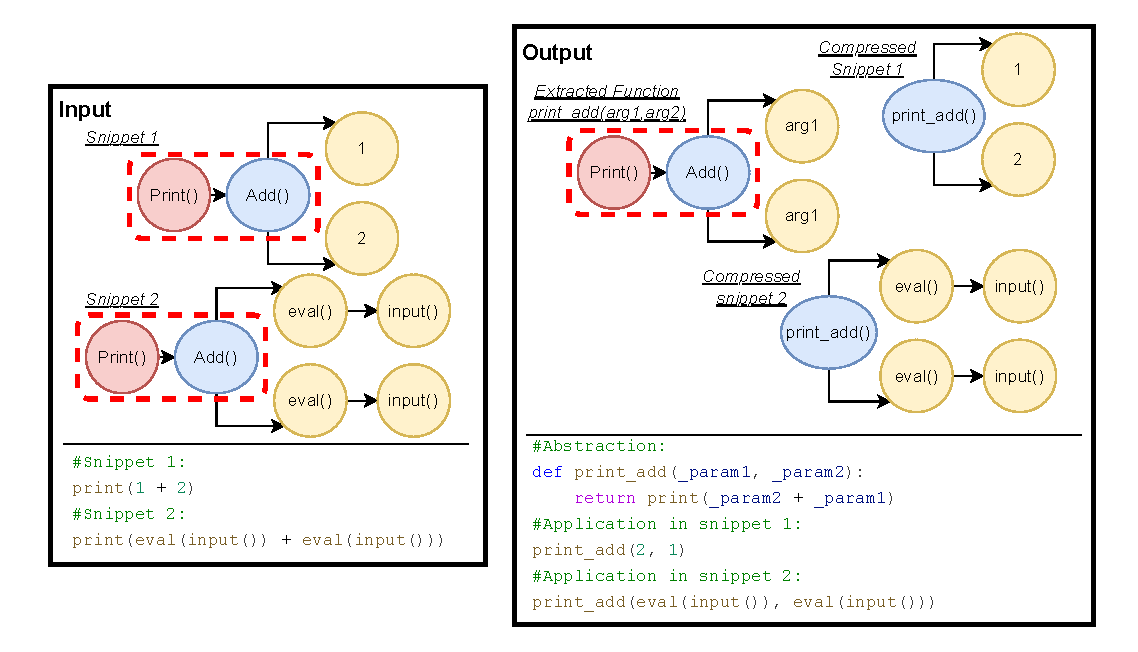
\includegraphics[width=\linewidth]{images/LibAbsAST.pdf}
  \caption{A library extraction example showing snippets of the input code, the output code, and their ASTs. The corpus (left) comprises of two code snippets who share a common structure (highlighted). CTS can extract this common structure, here named \code{print\_add(arg1,arg2)}, and replace it with a function call (right).  }
  \label{figure:LibAbsAST}
\end{figure}

\subsection{Corpus Guided Top-down Search}
Corpus Guided Top-Down Search (CTS) is a recursive search method~\cite{Bowers_2023stitch} that looks for the optimal function, with respect to some utility measure, to be extracted from a given corpus. The algorithm starts with the search target of a partial program tree, naively an empty tree, and it searches the corpus for matching partial sub-trees. The target's utility is then computed based on the number of matches found and the target's size, where larger targets with more matches have higher utility. In each subsequent round, the target is updated by adding child nodes to its leaf nodes. This expands the target, but consequently reduces the matches. The children are added depending on the corpus, as well as the expected utility. That is, the utility of expanding some branches of the target can be bounded by the current optimal utility, which guides the search to expand the target elsewhere. The search is concluded when the target reaches the optimal utility. The target then becomes the body of the extracted function, and the leaf's children not included in the extracted function become the function's arguments. Figure \ref{figure:LibAbsAST} shows an example of CTS function extraction.  % JI: why left-out?  do we just mean the target's children?

% Top-down search starts with a small incomplete program, na
% Stitch extracts a library from a given program corpus by performing a corpus-guided top-down search (CTS) over the program's AST to find the optimal repeated sub-trees. In CTS, the search starts from the top with an empty program.  anwhere some AST nodes are included but their children are not. The omitted children represent search holes to be filled.\todo{explain the hole/topdown search thing 41:4,5} Stitch speeds up the library abstraction process by doing a utility-based CTS where it computes the utility of common sub-trees, and prune the search space to eliminate search paths that are guaranteed to have a lower utility than the current optimal one. The abstraction utility is calculated based on the size of the abstracted sub-tree and its useage frequency. Meaning abstracting complex functionalities that are more frequently used in the given corpus is prioritized over abstracting smaller ones or ones not frequently used. 
% }

% DreamCoder~\cite{ellis2020dreamcoder} is a State-of-the-art program synthesizer where the agent ( the synthesizer) is given a corpus of programs to learn from. Instead of synthesizing code directly, the agent first abstracts a library of repeated functionalities over the given corpus thus compressing the corpus. This reduces the agent's error probabilities by reducing the size of the code the agent has to write, as it can use the abstracted functions instead of rewriting them whenever needed. Hence, to speed-up program synthesis, one could speed up library abstraction. Library extraction involves identifying and extracting the repeated functionalities from a corpus, which is facilitated by analyzing the Abstract Syntax Trees (ASTs) of the programs. ASTs provide a structured representation of the code, allowing algorithms to identify common patterns or sub-trees that can be abstracted into reusable functions. Stitch~\cite{Bowers_2023stitch} is a State-of-The-Art library abstraction tool that takes in a list of programs written in a lisp-like syntax and outputs a library (a list of abstracted functions) while also re-writing the input programs to utilize the abstracted functions. It does so by performing a corpus-guided top-down search (CTS) over the programs' Abstract Syntax Trees (ASTs) to find the optimal repeated sub-trees. ASTs provide a structured representation of the code, allowing algorithms to identify common patterns or sub-trees that can be abstracted into reusable functions. Consider a corpus of programs where multiple programs contain a similar sequence of operations to compute the factorial of a number. The library extraction process would identify this common pattern in the ASTs of these programs and abstract it into a reusable function \texttt{compute\_factorial(n)}. Stitch speeds up the library abstraction process by doing a utility-based CTS where it computes the utility of found common sub-trees, and prune the search space to eliminate search paths that are guaranteed to have a lower utility than the current optimal one. The abstraction utility is calculated based on the size of the abstracted sub-tree and its useage frequency. Meaning abstracting complex functionalities that are more frequently used in the given corpus is prioritized over abstracting smaller ones or ones not frequently used. 

%-------------------------------------------------------------------------------
% \subsection{Motivation} % maybe rename. 
% % JI: we can cut this for space.  It repeats the introduction and doesn't really add anything.
% Library extraction for general purpose languages is important in that it enhances code reuse, allowing developers to avoid redundancy, thereby saving time and effort in software development. This practice helps with consistency and standardization across a corpus of code, as common functionalities are centralized in libraries rather than duplicated across multiple areas within the corpus. Additionally, library extraction facilitates maintenance and debugging; by isolating functionalities into discrete libraries, updates and bug fixes can be applied uniformly, just by applying them to the abstracted functions, reducing the risk of inconsistencies and errors. It also fosters modularity, enabling developers to build and extend applications more flexibly by integrating standalone components. This approach not only accelerates the development process but also improves software quality and reliability, as libraries often undergo rigorous testing. Ultimately, the motivation for library extraction lies in creating efficient, maintainable, and scalable software systems.






%-------------------------------------------------------------------------------
% \todo{everything down here is the second or 3rd paragraph of 3 ( 3.1 Problems)}
% \todo{Add some sentences about why it is interesting to lift stitch to python. Something about how developers would find it useful to have such a tool.}

% it can be augmented with a python-lisp compiler and a decompiler. The compiler would transform the inputted python programs to the lisp-like format that is passed to Stitch. \toolname then decompiles the output of Stitch back to python. 

% %-------------------------------------------------------------------------------
% \section{Design }
% %-------------------------------------------------------------------------------
% % a concrete proposal for how you intend to complete the project


% \begin{figure*}
%   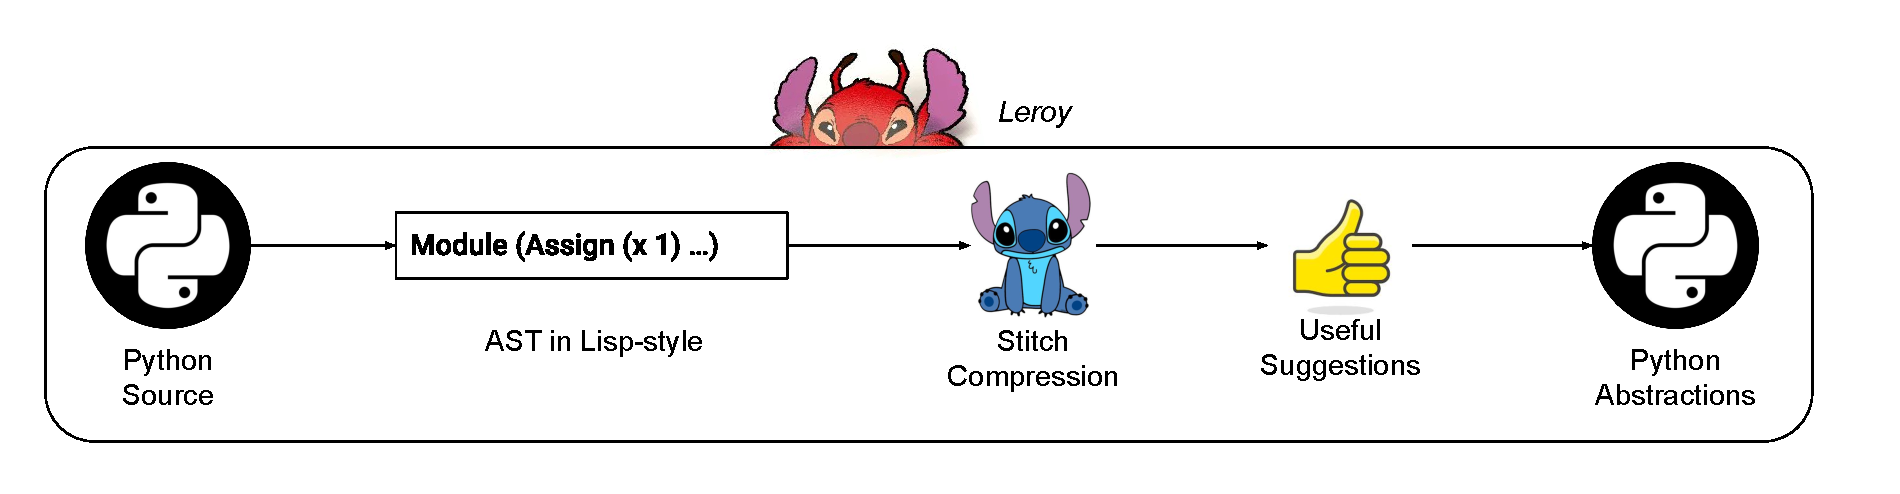
\includegraphics[width=\textwidth]{images/Design.pdf}
%   \caption{\toolname's high level design}
%   \label{fig:design}
% \end{figure*}
% \toolname performs library extraction by operating on the AST of the programming language. \toolname uses Stitch \cite{Bowers_2023stitch} as the library extraction engine, prunes invalid abstractions produced by it to present the most useful suggestions to the developer. Figure \ref{fig:design} shows the high level design of \toolname.
% % In the sections below, we describe each step in detail.

% \subsection{Representing Program AST in a lisp-like form}
% To convert program \textbf{ASTs to Lisp}, we treat ASTs as a series of nested function calls, with nodes as the function and subsequent child nodes as the argument of the function. This enables us to unwrap the AST into one long function call.
% % \todo{Add diagram of AST and converted lisp?}

% \subsection{Pruning Invalid Abstractions}
% Stitch suggests abstractions which involve language expressions/statements as function parameters. To \textbf{enhance abstractions} from stitch, we prune such cases. 


% \subsubsection{Macro-Like Abstractions}
% To prune macro-like abstractions, we attempt to convert the abstraction back into a program AST, and check if the tree is well-formed (all required children of a parent exist). Any incomplete ASTs are deemed to be macro-like and are pruned.

% \subsubsection{Invalid Parameters}
% We use a similar approach to find cases where invalid parameters could be passed to the abstraction. We convert the abstraction's body into a program AST and encode the abstraction's parameters as identifier nodes. 
% Then, we check if these identifier nodes are valid children in the AST. For example, an identifier node cannot be a valid child of a comparison expression's operator. But, an identifier node can be a valid child of the same expression's operand. 

% To summarise, if the AST is invalid or not well-formed, we deem the abstraction to be invalid.

% \subsection{Presenting Non-trivial Abstractions}

% To prune trivial abstractions (e.g. a function which performing addition of two arguments), we introduce a minimum size for the abstraction. This ensures that we have interesting abstractions coming out of \toolname.


% \subsection{Figuring out the return value}

% We augment the abstraction from Stitch by adding a necessary return value, if it does not exist. Our approach returns the last variable or expression in the abstraction's body. This is a simple approach that ensures that abstractions are functional in the target programming language. 

% % We remove abstractions which take language expressions/statements as parameters. 

% % \todo{This is the research problem. Add details when we have a more concrete solution.}

% % \subsection{Converting Lisp to Language AST}
% \subsection{Converting abstractions back to the PL}
% Finally, we convert the suggestions from stitch back into the AST. Then, we unparse the AST to result in the compressed code. 

% \todo{add design diagram.}

%------------------------------------------------------------------------------

\section{Design}
\label{sec:design}
Stitch~\cite{Bowers_2023stitch} uses a corpus guided top down search approach directly, which works on the lisp-like programs expected by Stitch, but the approach naively fails in less regular languages due to correctness issues: extracted common subtrees may not, in fact, be valid in the original language.

For example, when Stitch is given a Python's abstract syntax tree (AST) represented in a lisp style, 
% (tweaked to have a lisp-like lambda format) 
some elements or expressions, like the keywords "while" and "if", or operators like "==" and ">", are treated as first-class citizens of the programming language --- extracted subtrees could contain variables that hold such values, or functions could be called with these elements as parameters, resulting in syntactically incorrect calls, 
e.g.\ \texttt{compare(1,2,==)} or assignments, e.g.\ \texttt{x = while}.
% either variable names or function names depending the lamlispifying implementation.
Broadly, this issue arises because Stitch assumes a regular lambda calculus represented in a lisp style, and a Python AST is not sufficiently regular. 
% So, it has no knowledge of what would be a valid abstraction in a language like Python. 

% is unaware of the programming language it is abstracting over, but instead 
% This can result in incorrect abstractions, like an abstraction that expects "if" or "while" as arguments and treats them as variables. Hence, 
% To better generalize Stitch and extend it to a language like Python, we identify and prune such invalid abstractions. 
\toolname{} extends Stitch to correctly extract a library from a corpus of the language \ptwo{}, a large formal subset of Python 3 developed by Siek and Chang~\cite{pythonbook} in their textbook for compiler instruction. All \ptwo{} programs are valid Python 3 programs with equivalent behavior.  The \ptwo{} language supports imperative-style programming, with scoped variable assignment, control, function calls and non-nested definitions.  The language is dynamically typed across integer, booleans, lists, and dictionaries, with support for corresponding operations and comparisons.  Output is done through the \texttt{print} keyword, and input handled via a fixed expression \texttt{eval(input())}, which takes user input, represented as an unsupported string type, and casts it to the appropriate type (e.g.\  if the user inputs \texttt{``True''}, the return value of the corresponding \texttt{eval(input())} expression will be the boolean \texttt{True} value).  The full grammar of \ptwo{} is reproduced in the appendix.
% JI: we should remove lambdas?

The architecture of our \toolname{} tool is shown in Figure ~\ref{fig:design}. As input,
\toolname{} expects in a corpus of \ptwo{} programs.  In the first step (\emph{lispify}), it coverts the \ptwo{} programs into a lisp-like format recognizable to Stitch~\cite{Bowers_2023stitch}.  Stitch then proposes a lisp-like candidate for extraction.  The candidate is subsequently subjected to a series of \emph{pruning} checks that verify that the candidate can, indeed, be converted into a valid \ptwo{} function.  These checks correspond with a variety of issues that arise from Python's lack of regularization, and we describe them in depth in the following sections.  Once the candidate is verified, we use liveness analysis to add necessary parameters and return values --- this \emph{closing} is needed to handle the scope of live-in and live-out values from the candidate.  The final step is to \emph{pythonize} by converting the candidate back to standard \ptwo{} and adjusting the corresponding call sites.

In the following subsections, we cover each step of the \toolname{} pipeline in detail.



\begin{figure*}
  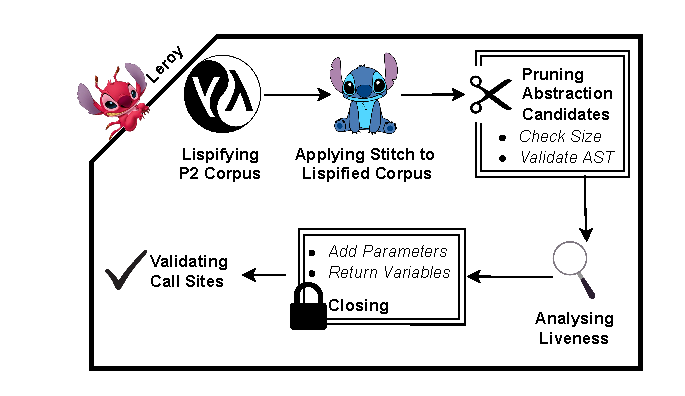
\includegraphics[width=\textwidth]{images/Design2.pdf}
  \caption{Architecture of the \toolname{} tool}
  \label{fig:design}
\end{figure*}

\todo{add the new more detailed figure}
\subsection{Problems}
\toolname extends Stitch by resolving \todo{six} main issues that arise when naively passing a lisp-like python AST to Stitch: 


\begin{enumerate}
    \item Trivial Abstractions:
    Because stitch optimizes on the abstracted function size relative to its use, it may abstract highly repeated single-line functionalities. This is \tocheck{because: such functionality is found in abundance within the code-base, and, there are no other larger abstraction candidates}. This results in functions that, for example, simply adds two numbers. \toolname eliminates such abstractions by imposing a lower constraint on abstraction size.
    \item Macro-like Abstractions: 
    Stitch treats abstracted libraries like macros\tocheck{, as it knows no better than to treat all program elements as first-class citizens}. When a functionality is abstracted, it can simply be swapped with a call. This approach impacts program correctness as it results in incomplete abstractions, like abstracting "exp + " from exp+exp. A potential abstraction $add(exp)$ would replace an addition of $1+2$ with the call $add(1) 2$. This is clearly invalid syntax.
    
    \toolname resolves this by reconstructing the AST in Python and checking its validity. 
    % To eliminate such abstractions, \toolname reconstructs the python AST from the suggested abstractions, and eliminate suggestions that fail to reconstruct a correct AST.  
    \item Invalid Parameters:
    The search method of stitch treats all tree nodes as potential "holes", or function parameters, which is incorrect in the case of python whose AST nodes are not all first-class citizens. For example, when stitch abstracts over comparative sub-trees, like "x == y" or "x!=z" it can suggest abstractions that takes three parameters, two operands and a comparison operator. A potential abstraction $f(x,op,y)$ would need to be called like: $f(x, ==, y)$ or $f(x, !=, y)$. This is clearly invalid syntax.
    
    \toolname also resolves this by reconstructing the AST in Python and checking its validity. 
    \item Incomplete return set:
    Because Stitch treats abstractions as macros, it does not consider variable scoping in abstractions, which impacts code correctness in a language like python. For example, Stitch can abstract assignments without returning the assignment targets. That is, it can suggest functions that change the value of a variable, but never returns the changed variable. In python, such assignment will create a new variable local to the abstracted (called) function instead of changing the value of the variable from the calling function. This, although syntactically correct, changes the program behaviour. \todo{To address this issue \toolname performs a liveness analysis to determine what variables are live out of the abstraction call, and returns those.}

    \item Incomplete Parameter Set:
    Some abstractions may use a variable that is not defined in the abstraction scope. This maybe because the same variable name is used in similar code-fragments across the corpus. As a result, that variable doesn't become a parameter to the abstraction.  
    To find these variables \toolname performs a liveness analysis to determine variables that aren't live into the abstraction's body. It is assumed that these variables exist in the calling scope, and they are added as parameters to the abstraction.

    \item Validating the correctness of call sites:

    Some abstraction calls may be invalid, as parameters passed to the abstraction may need to be recomputed within the abstraction's body. 
    Although we are able to find macro-like abstractions which are not valid python ASTs, these abstraction calls are still be macro-like.
    To validate the correctness of call-sites, we check that no parameter's expression is killed inside the abstraction. \toolname removes such abstraction calls.

\end{enumerate}





% \toolname performs library extraction by operating on the Abstract Syntax Tree (AST) of a subset of Python. It compiles a python AST into a lisp-like syntax that adheres to Stitch's grammar, then utilizes Stitch \cite{Bowers_2023stitch} as the library extraction engine, \toolname prunes invalid abstractions produced by Stitch to present the most useful suggestions to the developer, and compiles the output back to a python AST. Figure \ref{fig:design} illustrates the high-level design of \toolname.



\subsection{Lispifying}
To use Stitch, \toolname must first convert the \ptwo{} program into a Lisp-like representation. 
This conversion treats AST nodes as nested function calls, where each node acts as a function and its child nodes as arguments. This approach enables \toolname to unfold the AST into a single, unified function call, simplifying the abstraction process. For instance, consider an AST representing \tocheck{the addition operation $1+2$. The AST would look like a tree, with an 'add' node at the root and $1$, $2$ as it's children. Refer figure \ref{figure:LibAbsAST} for a depiction. We can also represent the tree as this function call `add(1, 2)`, where the left and right children are the first the second operands respectively.}. In Lisp-like form, this would appear as `(add 1 2)`. 

\tocheck{Additionaly, \toolname lispifies a list of statements (like a function's body) as a cascading list of function calls. As an example, consider the following three statements $x=1$, $y=1$, $print(x+1)$. \toolname encodes this as $StatementList(x=1, StatementList(y=1, StatementList(print(x+y), \epsilon)))$, where $\epsilon$ is the empty statement. This encoding draws inspiration from the `let` statement in Lisp. We do this to allow statements in the middle of a function to be abstracted. This is a crucial step in the encoding process that allows the creation of many more abstractions.
As a result, Stitch is capable of suggesting abstractions like $StatementList(x=1, StatementList(y=1, ?))$, where the $?$ is a parameter to the abstraction. In this case, the statement list $StatementList(print(x+y), \epsilon)$ would be passed as a parameter. \toolname ensures to pluck out this extra argument and place the statement back in the abstractions calling scope.}

After utilizing Stitch, \toolname converts the lisp-like syntax to a python AST which can then be unparsed to correct python code. 


\subsection{Pruning Stitch's Abstractions}
Stitch suggests many abstractions that may not port well to Python. To refine these abstractions, \toolname employs pruning strategies. Other valid abstractions are augmented with additional information, such as adding return statements, or accepting more parameters in the abstraction's signature. 

\subsubsection{Macro-Like Abstractions}
To identify and prune macro-like abstractions where the abstraction is an incomplete python code, \toolname attempts to reconstruct the abstraction into a program AST form, then checks for the correctness of the yielded AST. It verifies the completeness of the AST by ensuring all required child nodes of a parent node exist. Incomplete ASTs are indicative of macro-like structures leading them to be subsequently pruned. For example, an incomplete AST might involve a function call without required arguments, such as `(add a)` where `b` is missing. 

\subsubsection{Invalid Parameters}

Additionally, \toolname identifies cases where abstractions incorporate invalid parameters. It analyzes the abstraction’s body by converting it back into a program AST and encoding parameters as identifier nodes. By validating these nodes against the AST structure, \toolname ensures the legitimacy of parameter usage within the abstraction. For instance, in a comparison expression `(a > b)`, Stitch may produce an abstraction of the form \texttt{compare(a, comparator, b)} instead of \texttt{greater\_than(a,b)}. Such abstractions that take in invalid parameters are pruned out. 

\subsubsection{Presenting Non-trivial Abstractions}

To enhance the utility of suggested abstractions, \toolname filters out trivial cases by imposing a minimum size requirement. This criterion ensures that the extracted abstractions are sufficiently complex and meaningful to warrant inclusion. This enforces trivial functions, like simple addition or printing, are not abstracted alone despite having a high utility due to its high usage frequency. 

\subsubsection{Determining the Return Value}

\toolname complements the abstractions generated by Stitch by ensuring a coherent return value, if absent. 

To find what needs to be returned, \toolname performs a liveness analysis, to determine what variables are live out of the abstraction body. This is done by examining the target site of the abstraction. 
It is worth noting that the abstraction's parameters may themselves be live-out and need to be returned. 

If there are no live-variales out, \toolname reverts back to returning the last variable or expression in the abstraction’s body. 

Such an approach helps with functional correctness of the abstractions in the target programming language. For example, Stitch may produce an abstraction where a variable is updated, but does not return the variable at the end of the abstraction, thereby generating erroneous compressed code. 

\subsubsection{Determining Additional Parameters}:

Stitch's abstractions may assume the presence of certain variables, even if they aren't passed into the abstraction. This is because the same variable names appear in similar code-fragments across different parts of of the corpus. It is important to pass these as parameters to have a valid python function. We find variables that are \textit{not} live into the abstraction's body and add them as parameters. 

\subsubsection{Validating the correctness of call sites}
\toolname also checks the validity of each abstraction call, to ensure that the call doesn't change the code's functionality. As Stitch treats abstraction parameters like macros, there maybe parameters whose values need to be recomputed in the abstraction's body. 

This is best illustrated with an example. Consider the abstraction in figure \ref{fig:possible-invalid-function-call}. This function prints the value $param0$ in a loop that runs 5 iterations.

Stitch detects that this abstraction could be called at \ref{fig:invalid-targetsite}, by using the function call $func1(x+5)$. However, this is an invalid call as x+5 is re-computed every iteration in the loop; but the passing the value as $param0$ computes it only once at the call site. This changes the code's behaviour.

To detect such invalid call-sites, \toolname analyses the target site to determine that the expression $x+5$ is killed within it. As a result, the expression cannot be computed once, at the start of the target site; making this an invalid abstraction call.

In general, we determine if any parameter passed will be killed inside the body of the abstraction. If so, we deem such an abstractio call to be invalid.

\begin{figure}
    \begin{lstlisting}
    def func1(param0):
        for x in range(5):
            print(param0)
    \end{lstlisting}
    \caption{A valid function, which could be called erroneously}
    \label{fig:possible-invalid-function-call}
\end{figure}

\begin{figure}
    \begin{lstlisting}
    for x in range(5):
        print(x+5)
    \end{lstlisting}
    \caption{An invalid target site for func1}
    \label{fig:invalid-targetsite}
\end{figure}

\begin{figure}
\begin{lstlisting}
    -> func1(x+5) 
\end{lstlisting}
    \caption{An invalid call site to func1}
    \label{fig:invalid-callsite}
\end{figure}


\subsection{Pythonizing}
Finally, ASTs are converted back to python using the `ast.unparse` function.

% \subsection{Converting Abstractions back to the Programming Language AST}

% Finally, \toolname converts the refined suggestions from Stitch back into the Abstract Syntax Tree of the programming language. It then unparses the AST to yield the compressed code, integrating the identified abstractions seamlessly into the original program structure.


%-------------------------------------------------------------------------------

\section{Evaluation}
\label{sec:eval}


We developed \toolname with Stitch commit number \todo{6fa2...} and we evaluate it on a \todo{xyz} machine running a \todo{xyz} operating system version \todo{xyz}. To evaluate it, we used a corpus of \todo{50} python programs \todo{maybe cite a github link to P2 test cases} that adhere to the P2 grammar described in figure \ref{fig:grammar}. The testing corpus can be found on \todo{github link)} along with \toolname's code. 

Applying Stitch, with no pruning or validation, on lispified input yields \todo{15} total abstracions. Out of which \todo{5} of the \todo{15} found abstractions were trivial, \todo{3} involved macro-like statements, \todo{5} took in invalid parameters and only \todo{2} were valid abstractions. In comparison, applying \toolname to the same input, with the minimum size threshold set to \todo{20} outputs 6 valid abstractions, some of which create and return functions. We found that each abstraction was applied with \todo{3} call sites on average. We compressed the code by \todo{X}.

\todo{what are the other parameters passed in the testing process?}

\todo{rename to methodology? include limitations here? }
% This shows the necessity of our techniques. 

% \toolname is able to find 6 abstractions, after applying our techniques. We used a minimum threshold size of \todo{20} \todo{size unit} to ensure larger sized abstractions. Notably, \toolname was also able to find abstractions that created and returned a function. 





\todo{machine ?}
\todo{Discuss the impact of our pruning methods on utility }
%-------------------------------------------------------------------------------

\section{Related Work}
\label{sec:relwork}
%-------------------------------------------------------------------------------
% \todo{Section 6, merging all group members drafts, below are the individual drafts}

% Abhiram: 
% \textbf{Program synthesis} aims to auto-generate programs that meet input-output requirements. Most techniques utilise a specialised DSL(domain specific language) to make the synthesis faster and more tractable. 
% Dreamcoder\cite{ellis2020dreamcoder} and EC2 \cite{EC2} lead a line of work\cite{laps, LILO, EC, MCMC} in inductive program synthesis, which takes inspirations from the way humans write code: developing reusable libraries. 
% These techniques take a set of tasks(ex: input, and corresponding outputs), and aim to synthesise programs at meet the task's specifications. To achieve this goal, a two-step process is followed. First, the technique partially synthesises a suite of programs that accomplish the tasks. Then, it learns reusable elements(libraries) from these programs which are further used to enhance the quality of synthesis. 
% % Specifically, DreamCoder uses an EC\textsuperscript{2} (Explore, Compress, Compile) ~\cite{EC2} synthesis algorithm, where it abstracts libraries in one of its 2 sleep stages to explore potential extensions to the given corpus, then compress the found abstractions in the next sleep stage to grow the library used for training the recognition neural network and synthesize programs in the wake stage of the next cycle. However, DreamCoder's success in solving problems in various domains, such as physics laws and text-editing, came with very high time cost. 
% This line of work is designed, or evaluated for learning abstractions over programs written in domain specific languages or lambda calculus. 
% % \todo{It is unclear how these techniques extend to higher-level languages.}
% % LILO uses LLMs to documentation, functional languages.
% % \todo{Add citations to LAPS, LILO, EC2, EC}

% Some works\cite{regal, patios} aim to extend these techniques to high-level languages. PATOIS \cite{patios}, equips and trains a neural synthesizer to use learned code idioms, while Regal\cite{regal} utilises LLMs to synthesise and abstract programs. Both of these techniques do not specifically aim to learn better abstractions.
% % These techniques are primarily 

% \textbf{Learning Abstractions:} 
% % that are useful and repeated in a corpus of programs is the goal of \cite{shapecoder, shapemod, babble, stitch}. 
% Babble\cite{babble} and Stitch\cite{stitch} are two closely related works that focus entirely on library extraction. While babble aims to improve the quality of learned libraries by using e-graphs and rewrite rules, stitch provides guarantees on the size of the learned corpus and the speed at which libraries are learned. 
% ShapeMod\cite{shapemod} and Shapecoder \cite{shapecoder} learn useful and explainable macros by limiting to programs that draw 3D shapes.
% % This line of work is designed, or evaluated for learning abstractions over domain specific languages(such as drawing shapes), or functional programming languages.
% Our work aims to extend these ideas to high-level languages like Python.


% An \textbf{Extract Method refactoring} \cite{jdeo, jextract, gems} aims to extract reusable blocks of code from a function. While these techniques operate on languages commonly used by software developers(Java), most have a limited vision: only the function to be modified is taken into account. In contrast, library learning techniques such a babble\cite{babble} look at the entire corpus of programs as a whole, with the potential to discover abstractions by correctly rewriting programs. 


\subsection{Program synthesis}
Library Abstraction aims to compress code via extracting common functionalities of multiple functions into a single repeatedly used function. However, this is usually done with the bigger goal of generating better libraries to be used for program synthesis (the generation of programs that solve a given problem). Most current state-of-the art work on library extraction are based on DreamCoder~\cite{ellis2020dreamcoder}, a program synthesizer that adopts the wake-sleep algorithm~\cite{wake-sleep} to bootstrap inductive program synthesis from a small problem-corpus represented with a Domain Specific Language (DSL). Specifically, DreamCoder uses an EC\textsuperscript{2} (Explore, Compress, Compile)~\cite{EC2} synthesis algorithm, where it abstracts libraries in one of its 2 sleep stages to explore potential extensions to the given corpus, then compress the found abstractions in the next sleep stage to grow the library used for training the recognition neural network and synthesize programs in the wake stage of the next cycle. However, DreamCoder's success in solving problems in various domains, such as physics laws and text-editing, came with very high time cost. 

\subsection{Library Abstraction}
Subsequent work aimed to enhance DreamCoder through enhancing the abstraction methods. For example, Babble~\cite{Cao_2023babble} proposes utilizing semantics-based abstractions, which results in better abstractions in less time. However, Babble's efficiency comes with an input complexity cost. In addition to the program corpus, users must also input a semantic equivalence list, which the program uses to abstract common libraries over semantically equivalent programs that look different. Stitch~\cite{Bowers_2023stitch} on the other hand aims to efficiently abstract libraries by reducing the abstraction search space. It does so by defining a utility measure, and performing a top-down search that optimizes utility using the branch and bound method, which eliminates search branches that are upper-bounded by a utility smaller than the current best utility. 

\subsection{Using LLMs}
As discussed earlier, one aim of library abstraction is to enhance program synthesis, which requires the abstracted libraries to be properly documented, which Lilo~\cite{grand2024lilo} covers. To improve program synthesis, lilo utilizes Large Language Models (LLMs) to provide common sense knowledge as a first search step over the string space, before performing an enumerative search over the program space as in DreamCoder. Lilo then uses the Stitch compressor, and once more utilize LLMs to document the resulting libraries with a natural language. The use of the full lilo system enhances performance, in contrast to incorporating LLM guided search without the documentation phase which degrades performance. However, all aforementioned work take in \(lambda\)-calculus and DSL input, unlike ReGAL~\cite{stengeleskin2024regal} which similarly uses LLM-guided search and utilize LLMs in library generation and documentation, but also works with general purpose languages like python. However, ReGAL uses library extraction as a step in program synthesis, where its main goal is to synthesize programs that satisfy a given written task. 

\subsection{Visual Abstraction, Program Learning, and Rewriting}
Other work cover library abstractions with a focus on visual representation programs~\cite{jones2023shapecoder} ~\cite{wang2021learningVisAbst}~\cite{Jones_2021}. ShapeCoder ~\cite{jones2023shapecoder}  for example uses Neural Networks and e-graphs to not only extract useful abstractions from visual modeling programs, but also explain input shapes using the abstractions. 
Other lines of work, despite not sharing the library extraction focus, share components of programming and natural language processing and recognition. This includes work on program learning~\cite{cropper2019playgol}~\cite{DBLP:journals/corr/abs-2004-09931refproginduc}~\cite{wong2022leveraging}  ~\cite{demo}~\cite{iyer2019learning} ~\cite{hocquette2024learning} and program rewriting~\cite{brandfonbrener2024verified} ~\cite{DBLP:conf/sat/NotzliRBNPBT19rewrite}~\cite{ganeshan2023improving}, which use relevant methods such as finding idioms, and search algorithms as the Monte Carlo tree Search. 


\section{Discussion and Future Work}
\label{sec:conc}

Although \toolname generalizes Stitch \cite{Bowers_2023stitch} and addresses 
the main issues Stitch has when fed with python code, it has yet to be more extensively and rigorously tested, 
as well as compared against other previous work. Prior to testing, \toolname can also be extended further to better address 
the stated problems with more advanced program analysis methods, to optimize the current solutions approaches. Furthermore, \toolname extends Stitch without utilising program semantics as babble~\cite{Cao_2023babble} does. Hence, \toolname can be enhanced by adopting from babble and utilizing semantic equivalence to expand the abstraction choices. Lastly, currently \toolname is only tested for compression, but library abstraction for python also targets readability and other program quality metrics that can be encoded in the utility function, and are yet to be tested. 
% \todo{say something about extending from p2 to entire python}



% \begin{enumerate}
%     \item Integration of babble and stitch
%     \item Extension of evaluation
%     \item Comparison against other related work: Regal (novelty), extract-method tools, ast-based code clone detection. Check other work form ICSE/FSE.
%     \item Thoughts about what would make this a full research paper
% \end{enumerate}

% Additionally, \toolname ensures that abstractions involve parameters that are data types.

% Match locations only contain valid function calls.

% Implementation in on ast-completing checking in Rust

% Find a way to measure usefulness/how interesting an abstraction is.

% % % Bibliography
\bibliography{references}
% \bibliography{\jobname}

% %%%%%%%%%%%%%%%%%%%%%%%%%%%%%%%%%%%%%%%%%%%%%%%%%%%%%%%%%%%%%%%%%%%%%%%%%%%%%%%%
% \end{document}
% %%%%%%%%%%%%%%%%%%%%%%%%%%%%%%%%%%%%%%%%%%%%%%%%%%%%%%%%%%%%%%%%%%%%%%%%%%%%%%%%

%% Appendix
\appendix
\FloatBarrier
\section{Appendix: \ptwo{} Grammar} 
\label{sec:grammar}
\toolname operates on a subset of Python 3 named \ptwo{} as described in ``A Problem Course in Compilation: From Python to x86 Assembly''~\cite{pythonbook}. \ptwo{} consists of integer and boolean values and variables, addition and subtraction, boolean operations, comparators, conditionals and ternaries, while loops, and function calls and definitions. The grammar of \ptwo{} is given below.

\begin{figure}
\begin{lstlisting}
program ::= module
module ::= statement+
statement ::= simple_statement | compound_stmt
simple_statement ::= "print" "(" expression ")"
                   | target "=" expression
                   | expression
                   | "return" expression
                   | name "=" expression
expression ::= name | decimalinteger
             | "True" | "False"
             | "-" expression
             | "not" expression
             | expression "+" expression
             | expression "and" expression
             | expression "or" expression
             | expression "=="
             | expression "!="
             | expression "if" expression "else" expression
             | expression "is" expression
             | "(" expression ")"
             | "[" expr_list "]"
             | "{" key_datum_list "}"
             | subscription
             | expression "[" expression "]"
             | expression "(" expr_list ")"
             | "eval" "(" "input" "(" ")" ")"
subscription ::= expression "[" expression "]"
target ::= identifier | subscription
key_datum ::= expression ":" expression
key_datum_list ::= key_datum | key_datum "," key_datum_list
expr_list ::= expression | expression "," expr_list
id_list ::=identifier | identifier "," id_list
compound_stmt ::= "def" identifier "(" id_list ")" ":" suite
suite ::= "\n" INDENT statement+ DEDENT
name ::= identifier
decimalinteger ::= [0-9]+
\end{lstlisting}
\label{fig:grammar}
\caption{P2 Grammar}
\end{figure}

\newpage


\section{Appendix: Abstractions found by \toolname} 
The complete list of abstractions found by \toolname:

\begin{figure}
    \begin{subfigure}[t]{0.45\textwidth}
        \begin{lstlisting}[language=Python, firstnumber=1]
def swap_print(_param0, _param1,
    _param2, _param3):
    _param1 = _param3
    _param0 = _param2
    print(_param1)
    print(_param0)
    tmp = _param1
    _param1 = _param0
    _param0 = tmp
    print(_param1)
    return print(_param0)
        \end{lstlisting}
        % \caption{Function 1}
        \label{fig:func1}
    \end{subfigure}\hfill
    %
    \begin{subfigure}[t]{0.45\textwidth}
        \begin{lstlisting}[language=Python, firstnumber=1]
def assign_add(_param0, _param1,
    _param2, _param3):
    if int(_param3):
        _param1 = _param1 + _param2
    else:
        _param1 = _param1 + _param0
    return _param1
        \end{lstlisting}
        % \caption{Function 2}
        \label{fig:func2}
    \end{subfigure}
    
    \vspace{0.5cm} % Adjust vertical space between rows
    
    \begin{subfigure}[t]{0.45\textwidth}
        \begin{lstlisting}[language=Python, firstnumber=1]
def assign_print( _param0, _param1,
    _param2,_param3):
    _param1 = _param3
    _param0 = _param2
    return print(_param1 + _param0)
        \end{lstlisting}
        % \caption{Function 3}
        \label{fig:func3}
    \end{subfigure}\hfill
    %
    \begin{subfigure}[t]{0.45\textwidth}
        \begin{lstlisting}[language=Python, firstnumber=1]
def if_print(_param0, _param1,
    _param2, _param3):
    if _param3(_param2):
        print(_param1)
    else:
        print(_param0)
        \end{lstlisting}
        % \caption{Function 4}
        \label{fig:func4}
    \end{subfigure}
    
    \vspace{0.5cm} % Adjust vertical space between rows
    
    \begin{subfigure}[t]{0.45\textwidth}
        \begin{lstlisting}[language=Python, firstnumber=1]
def multi_assign(_param1, _param2,
    _param3):
     x = 1
     y = 2
     z = _param3
     _param2 = _param1
     return (_param2, x, y, z)
        \end{lstlisting}
        % \caption{Function 5}
        \label{fig:func5}
    \end{subfigure}\hfill
    %
    \begin{subfigure}[t]{0.45\textwidth}
        \begin{lstlisting}[language=Python, firstnumber=1]
def multi_assign_2( _param1, _param2,
    _param3, x):
    y = _param3 + x
    z = _param2 + y
    w = _param1 + z
    return (w, y, z)
        \end{lstlisting}
        % \caption{Function 6}
        \label{fig:func6}
    \end{subfigure}
    
    \vspace{0.5cm} % Adjust vertical space between rows
    
    \begin{subfigure}[t]{0.45\textwidth}
        \begin{lstlisting}[language=Python, firstnumber=1]
def assign_print_eq(_param0, _param1):
    x = _param1
    y = _param0
    return print(x == y)
        \end{lstlisting}
        % \caption{Function 7}
        \label{fig:func7}
    \end{subfigure}
    
    \caption{Abstractions found by \toolname}
    \label{fig:leroy-abstractions}
\end{figure}

\end{document}